% !TEX root = ../../book.tex
\chapter{Execution Strategies\label{chap:ch_exec_models}}

While algorithmic trading techniques are useful in both low and high frequency settings, their importance has become more pronounced in the age of electronic trading because of the speed in execution and the necessity for efficient matching of demand and supply sides in the limit order book. Added to this is that modern equity markets where order submission and cancellations are automated and are also highly fragmented with dozens of exchanges and about forty alternative trading systems where investors can choose to trade. The trading algorithms also differ over various types of market participants, but all of them have common objectives, that is to optimize dynamically where, how often and at what price to trade. The algorithms have small reaction times to changing liquidity and price. Typically, the execution has been broadly classified into the following layers.
	\begin{itemize}
	\item \textbf{Macro Level:} Given a meta-order (parent trade) translate the objective function of a strategy into a trading schedule; when the algorithm should trade, in what size (child order), for how long and the spread of trading.
	\item \textbf{Micro Level:} Given a slice (child order) of the meta-order to trade, this layer of algorithm decides whether to place it as a market or as a  limit order and at what price level.
	\item \textbf{Smart Order Router:} For a given order (quantity and price level) to which venue should the order be sent. This part covers the so called space dimension.
	\end{itemize}


In this chapter we discuss these and other execution issues in the high frequency trading context. Generally the objectives of equity trading are to minimize the probability of making errors---minimizing the trading impact and avoiding adverse selection. In order to achieve high completion rates, the trading should operate with speed and necessary risk control. It has to be noted that the average trade size has come down over time; thus the parent orders are increasingly decimated and are sent to the exchanges as small child orders. Handling this with large parent order sizes with the focus on short-term alphas requires a great deal of trade timing insights.  


The execution agencies engage in providing pre-trade advice and post-trade reporting. The pre-trade advice include the estimation of market impact cost covered in Chapter~\ref{chap:ch_mi_models} and the post-trade reporting is useful for evaluating how well the agency's execution algorithm has performed as compared to some benchmarks. These include the fill rate, the fill composition (passive values aggressive covering the spread) and the evaluation measures such as the magnitude of price revision against the order after the trading ends. Different clients are likely to put different emphasis on these measures. 


These algorithms have been generated over time and they depend on how the complexity in trading has grown. In the first generation algorithms focus on trading at fixed rate over a time-aggregated interval, trading at a fixed participation rate and trading such that the average execution price is closer to market volume-weighted average price. The second generation algorithms focus on market impact and risk. The methods here are formalized similar to Markowitz's portfolio theory. Increasing risk aversion generally leads to shorter execution with higher market impact. As more trades occur near the market close, risk averse clients may trade entirely at the closing auction. Finally, the third generation algorithms closely track the state of the limit order book and market data and are adaptive. The optimal decision such as updating the limit price, crossing the spread, cancellation of orders result from stochastic control formulation. The basic data used in these algorithms follow from microstructure signals covered in Chapter~\ref{chap:ch_trade_data_models}. 



\section{Execution Algorithms: Some Preliminaries}

The primary goal of most of the execution algorithms is to minimize the transaction costs which are broadly divided into direct costs and into indirect costs. The direct costs such as commissions, taxes etc are easy to measure and they primarily depend on quantity of trading. The indirect costs such as market impact and opportunity costs are hard to measure and depend upon trading strategies. Because many mutual fund and hedge fund companies engage in portfolio rebalancing periodically, they trade a large block of shares in a fixed duration. There is a trade-off between trading a large market order that is likely to affect the price adversely and splitting the parent order into many child orders and let the market recover after each trade. The modeling elements generally involve representing the permanent impact of a parent order and the temporary impact of trading a child order when the price normally returns back to equilibrium, short time after the trade, drift in price (alpha) and the volatility of the stock. The optimizing function balances the cost-loss in revenue due to price impact and the risk-uncertainty due to volatility of the underlying stock. If the trade occurs fast, we incur high cost and low risk but if the trade occurs slowly, we incur low cost and high risk.


The execution algorithms are generally evaluated through some benchmark prices. Some key quantities are:
	\begin{enumerate}[--]
	\item Arrival price, that is the market mid-quote at the start of parent order execution at $t=0$, $p_0$.
	\item Volume weighted average market price over the period of execution, $t \in (0,T)$, $p_{\text{VWAP}}= \sum_{i=1}^N V_ip_i/V$. \\ \\
	If the parent order of size, $X$ is split into `$n$' child orders with size, $x_k$, $k=1,\ldots,n$, then
	\item Volume weighted average price of the parent order's execution, $p_{\text{exec}}= \sum_{i=1}^n x_ip_i/X$. 
	\end{enumerate}
	
Two other related quantities that the traders examine in their evaluation strategies are:
	\begin{enumerate}[--]
	\item Slippage: $s= p_{\text{bench}} - p_{\text{exec}}$
	\item Market Impact: $p_0 - p_{\text{VWAP}}$
	\end{enumerate}
The execution cost is taken to be the slippage and the execution risk is its standard deviation. 


The influential paper by Kyle (1985)~\cite{kyle1985} argues that traders split the parent order to hide private information. The splitting of the order and how they are sent to the market, the strategies depend on the evolution of the stock price. These are broadly classified into static, one determined in advance of trading and into dynamic, one that depends on the state of the market. The static strategy under some conditions can also be dynamically optimal. Few commonly used criteria for allocation strategies are:
	\[
	\begin{split}
	&\text{VWAP: } x_k= X \cdot \dfrac{V_k}{V} \\
	&\text{Implementation Shortfall: Minimize }E(s)+\lambda \Var(s) \\
	&\text{Percentage of Volume: Minimize }\left(\dfrac{\text{Volume}_{\text{exec}}(x_k)}{\text{Volume}_{\text{market}}(v_k)} - v_{\text{target}}\right).
	\end{split}
	\]
These strategies as stated are static and they are based on a priori models for the evolution of price and volume traded over different times of the day. 


We present below select results in this area. The quantities that the trader can determine are the number of child orders $(n)$ and their sizes $(x_k)$ and the duration for the parent order trading $(T)$. The relevance of this problem to the practitioners is discussed in Chan and Lakonishok (1997)~\cite{lakon} and Keim and Madhavan (1997)~\cite{madhavan}. Bestimas and Lo (1998)~\cite{berlo} develop a model that suggests splitting the parent order to reduce the average trading costs. Almgren and Chriss (2000)~\cite{alm2000} split the parent order to minimize the mean-variance of trading costs similar to Markowitz's portfolio theorem. Some recent works on this topic are also briefly mentioned but, describe in some detail in the following sections.


\section{First Generation Algorithms\label{sec:first_gen}}

The performance of traders is evaluated by how they execute the orders in comparison to volume weighted average price (VWAP), because it is generally considered to be closer to how a passive trader would trade. Madhavan (2002)~\cite{mad_a02} warns that the uncritical use of VWAP are a benchmark can promote non-optimal trading behavior. As noted in the last section, other alternatives to VWAP as possible. The choice of a benchmark will obviously affect the placement strategies by the traders. Using daily VWAP as a benchmark leads to trades spread over the day and thus passive trading can significantly affect alpha. The pre-trade benchmarks such as the arrival price ignore the short-term trends in prices. The post-trade benchmarks are sensitive to order flows towards the end of the day and thus have higher price impact. The VWAP strategy can be automated so that order submissions can follow historical volume pattern during the course of the day with finer time grids. This practical approach is expounded in this section.


We will follow the formulation of the optimization problem as given in Busseli and Boyd (2015)~\cite{busseli_boyd}. With $X$, the total number of shares to be traded over the time horizon, $(0,T)$ in `$n$' discrete time intervals, the problem is to decide how to divide the parent order $X$ into child orders $x_1, \ldots, x_n$ so that the executed average price $p_{\text{exec}}$ is closer to $p_{\text{VWAP}}$. It is assumed that the price, $p_t$, is a random walk and thus the return is white noise. It is assumed that the trading algorithm mixes optimally market and limit orders. Defining the cost of trade in time interval $t$ as $x_t \hat{p}_t$, where $\hat{p}_t$ is the effective price that depends on the instantaneous transaction costs such as bid-ask spread with `$s_t$' as the fractional bid-ask spread with a certain participation rate $x_t/v_t$, it can be shown that the effective price is
	\begin{equation}
	\hat{p}_t= p_t \left(1 - \dfrac{s_t}{2} + \alpha \, \dfrac{s_t}{2} \cdot \dfrac{x_t}{v_t} \right),
	\end{equation}
which gives in the end quadratic transaction costs which is a reasonable approximation as seen from Chapter~\ref{chap:ch_trade_data_models}. Here `$\alpha$' is taken to be proportionally factor of market orders to total orders. Defining the proportional ratio
	\begin{equation}
	s= \dfrac{X p_{\text{VWAP}} - \sum x_t \hat{p}_t}{X p_{\text{VWAP}}}
	\end{equation}
as slippage, where the numerator is the cash flow to the broker, the optimizing function is
	\begin{equation} \label{eq:opt_function}
	E(s) + \lambda \Var(s).
	\end{equation}
Here `$\lambda$' is the risk-aversion parameter. It has to be kept in mind that the quantities $p_t$ and $v_t$ are random variables and the decision variable is `$x_t$'. Note with some approximation, $p_t \sim p_{t-1} \sim p_{\text{VWAP}}$ and with applying the law of iterated expectation, the optimization in \eqref{eq:opt_function} simplifies to
	\begin{equation}
	\min_{x_t} \sum_{t=1}^n \left[ \dfrac{s_t}{2x} (\alpha x_t^2 k_t - x_t) + \lambda \sigma_t^2 \left( \left( \sum_{r=1}^t u_r/X \right)^2 - 2 M_t \sum_{r=1}^{t-1} u_t \right) \right]
	\end{equation}
with constraints $x_t \geq 0$ and $\sum_{t=1}^n x_t= X$. Here the quantities $M_t= E \left[ \sum_{r=1}^{t-1} v_t/v\right]$ and $k_t= E[\frac{1}{v_t}]$ refer to market intra-day volume distribution. Assuming that the spread is a constant which is generally true for actively traded stocks, the optimal static solution can be shown to be equal to:
	\begin{equation} \label{eq:optimal_result_xt}
	x_t^*= X E\left(\dfrac{v_t}{v}\right), \enskip\enskip t=1,\ldots,n.
	\end{equation}
From the above discussion, it is clear that forecasting both the intra-day distribution of volume, $v_t$, and the total volume for the day, $v$, is essential for achieving optimal results. The optimal result in \eqref{eq:optimal_result_xt} can be obtained also with slippage as defined in the previous section. \\


\noindent\textbf{Bertsimas and Lo Model:} The basis of the model discussed here is that trading affects not only the current prices but also the price dynamics that affect the future trading costs. Thus the problem involves dynamic optimization but the solution turns out to be static. Assume that an investor wants to sell a parent order of $X$-shares in $(0,T)$, where $T$ is arbitrary, and let $x_k$ be the number of shares sold (child orders) with the realized price, $\widetilde{p}_k$. The cost of trading, also know as slippage is
	\begin{equation}\label{eqn:x7}
	s= Xp_0 - \sum_{k=1}^n x_k\widetilde{p}_k,
	\end{equation}
where $p_0$ is the arrival price. The model proposed in Bertsimas and Lo (1998)~\cite{berlo} can be stated as
	\begin{equation}\label{eqn:xk7}
	\min_{x_k} E_1 \left[\sum_{k=1}^n x_kp_k\right] \text{ such that }\sum_{k=1}^n x_k=X.
	\end{equation}
The criteria in (\ref{eqn:xk7}) call for determining the sizes of child orders a priori. To solve (\ref{eqn:xk7}), the model for price, where the price impact and price dynamics are separated, is taken to be,
	\begin{equation}\label{eqn:pk7}
	p_k = p_{k-1} - \theta x_k + \varepsilon_k,
	\end{equation}
where $\theta > 0$ representing the price impact and when $\theta = 0$, the model is simply a random walk model discussed in Chapter~\ref{ch:ch_uvts}. Under (\ref{eqn:pk7}) the best strategy for splitting the parent order, $X$, is shown to be
	\begin{equation}\label{eqn:equals}
	x_1^* = x_2^* = \cdots = x_n^* = \frac{X}{n},
	\end{equation}
the equal split. What the trader needs to decide a priori is the number of splits, $n$. The allocation strategy in (\ref{eqn:equals}) is termed as the time weighted average prices (TWAP) strategy in industry. 


The dynamic programming solution to (\ref{eqn:xk7}) via the so called Bellmann equations turns out to be elegant and simple because the price impact $(\theta x_k)$ does not depend upon the prevailing price $(p_{k-1})$ nor on the size of the unexecuted order $(X - \sum_{j=1}^{k-1} x_j)$. The indirect assumptions here are that the volume curve is even over different times of the day and the volatility profile is flat. Bestimas and Lo (1998)~\cite{berlo} also consider extensions of the model (\ref{eqn:pk7}), where a serially correlated state variable such as market condition (S\&P 500) is added. In this case it is shown that the best execution strategy at any point is a function of the state variable and the remaining unexecuted size. 


As a point of comparison to the equal allocation strategy observe that VWAP-strategy is similar in the sense that is does not also depend explicitly on any price movement. Simply the allocation is made in \eqref{eq:optimal_result_xt} can be intuitively justified as resulting from $\frac{x_k}{X}=\frac{V_k}{V}$. If the traders are restricted to only `$n$' time intervals, it is important to have a good forecast for the quantities, $V_k$ and thus, $V$, the total volume for the day. 



\section{Second Generation Algorithms\label{subsec:almchrmodel}}

\noindent\textbf{Almgren and Chriss Model:} The seminal paper by Almgren and Chriss (2000)~\cite{alm2000} and Almgren (2003)~\cite{almgren2003} consider the same problem taking into account the stock characteristics such as volatility via the mean-variance formulation of minimizing execution costs. This formulation treats the execution as a tradeoff between risk and cost; the faster the execution, higher the cost but lower the risk. The objective again is to liquidate, $X$ units before time `$T$' at minimum cost, in time steps, $t_k = k\tau$ for $k = 0,1,\ldots, n$ where $\tau = T/n$ is the average length of interval between successive child order submission times. If $X_k$ is the number of units held at $t_k$, the goal is to decide on the trading trajectory, $X_0,X_1,\ldots,X_n$ with $X_0=X$ and $X_n=0$. The number of units liquidated $x_k$ between $t_{k-1}$ and $t_k$ is called the trading schedule, with $x_k = X_{k-1} - X_k$. The trading strategy requires determining `$x_k$' in terms of information available at $t_{k-1}$. The static strategies determine the trading schedule in advance of starting trade time, $t_0$ and the dynamic strategies depend on information available up to $t_{k-1}$. Almgren and Chriss (2000)~\cite{alm2000} find trading trajectories that minimize $E(s)+\lambda \Var(s)$ for various values of $\lambda$.


The model for price impact is same as in (\ref{eqn:pk7}) but stated as
	\begin{equation}\label{eqn:bigpk}
	p_k=p_{k-1} - (\tau\theta)\dfrac{x_k}{\tau} + \sigma\tau^{1/2}\varepsilon_k,
	\end{equation}
where $v_k = x_k/\tau$ is the average rate of trading in $[t_{k-1}, t_k]$ and $\varepsilon_k$ are independent with mean zero and unit variance and `$\sigma$' is the volatility of the stock. The temporary impact represented by price per share received for sale in $[t_{k-1}, t_k]$ is
	\begin{equation}\label{eqn:pdouble}
	\begin{split}
	\widetilde{p}_k &= p_{k-1} - \eta\left(\dfrac{x_k}{\tau}\right) \\
			&= p_{k-1} - c \sgn(x_k) + \frac{\eta}{\tau}\cdot x_k,
	\end{split}
	\end{equation}
where $c$ can be taken to be fixed cost of selling which is the sum of mid-spread and fees. The temporary impact component is not present in the next period. Note (\ref{eqn:bigpk}) can be written as
	\begin{equation}\label{eqn:morepk}
	p_k = p_0 + \sigma\tau^{\frac{1}{2}}\sum_{j=1}^k\varepsilon_j - \theta(X - X_k),
	\end{equation}
and thus the shortfall
	\begin{equation}\label{eqn:longxeq}
	s = Xp_0 - \sum_{k=1}^N x_k\widetilde{p}_k = \sum_{k=1}^N \left(\frac{x_k}{\tau}\right) \eta - \sum_{k=1}^N \,[\sigma\tau^{1/2}\varepsilon_k - \theta x_k]X_k
	\end{equation}
is a function of the market volatility and the trade schedule, `$x_k$'. It captures the difference between the initial book value and the weighted average of realized prices. From (\ref{eqn:longxeq}), it follows that
	\begin{equation}\label{eqn:evardouble}
	\begin{split}
	E(s) &=  \theta\sum_{k=1}^N x_k X_k + \eta\sum_{k=1}^N \frac{x_k}{\tau} \\
	\Var(s) &= \sigma^2\sum_{k=1}^N \tau X_{k}^2\cdot
	\end{split}
	\end{equation}
If the trajectory is to sell at a constant rate, $x_k = \frac{X}{n}$ and $X_k = (n - k)\frac{X}{n}$, $k = 1,\ldots,N$,
	\begin{equation}\label{eqn:secondevardouble}
	\begin{split}
	E(s) &= \frac{1}{2}\theta X^2 + \varepsilon X + \left(\eta - \frac{1}{2}\theta\tau\right)\frac{X^2}{T} \\
	\Var(s) &= \frac{1}{3}\sigma^2X^2T(1 - \frac{1}{N})(1-\frac{1}{2N}).
	\end{split}
	\end{equation}
The trajectory minimizes expected cost but variance increases with $T$. On the other hand if we liquidate entire $X$ in the first time period,
	\begin{equation}\label{eqn:anotherdoubleex}
	\begin{split}
	E(s)&= c X + \eta \frac{X^2}{\tau} \\
	\Var(s)&= 0.
	\end{split}
	\end{equation}
If $n$ is large, hence $\tau$ small, $E(s)$ can be very large significant resulting in impact price.


 With these illustrations of extremes, the optimization problem can be restated as,
	\begin{equation}\label{eqn:minex}
	\min_x (E(s) + \lambda V(s)),
	\end{equation}
and if $\lambda>0$, $E(x)+\lambda V(x)$ is strictly convex and thus has a unique solution. The solution to (\ref{eqn:minex}) can be written as a combination of the exponentials. The results of trading trajectory and the trade list are given below:
	\begin{equation}\label{eqn:doublex}
	\begin{split}
	X_j &= \dfrac{\sinh (\kappa(T-t_j))}{\sinh (\kappa(T))}\cdot X, \quad j=0,\ldots,N \\
	x_j &= \dfrac{2 \sinh (\frac{1}{2}\kappa\tau)}{\sinh (\kappa(T))}\cdot \cosh(\kappa(T-t_{j-\frac{1}{2}}))X, \quad j=1,\ldots, n.
	\end{split}
	\end{equation}
Here $t_{j-\frac{1}{2}} = (j - \frac{1}{2})\tau$ and $\kappa = \sqrt{\lambda\sigma^2/\eta}$, that depends on the volatility and the risk aversion coefficient, `$\lambda$' is termed as urgency parameter. The inverse of `$\kappa$' is termed as the trade's ``half-life''; the larger its value the more rapid the depletion rate of the trade list. The solution given in (\ref{eqn:doublex}) is shown to be adaptive at any point in time, `$j$'. Thus the initial optimal solution over the entire interval is also optimal over each subinterval. A fixed trajectory as in (\ref{eqn:doublex}) was previously constructed by Grinold and Kahn (2000)~\cite{grin2000}. The closed form solution in (\ref{eqn:doublex}) is possible due to linear structure of impact functions. 


The value of `$\lambda$', the price of risk depends on the traders utility function. The suggested optimal strategy is just volume weighted average pricing (VWAP), that is trading at a constant rate, when $\lambda \to 0$, that is if the trader is risk-neutral. The trade schedule for various value of `$\lambda$' is given in Figure~\ref{fig:7first} and the projected execution schedule is given in Figure~\ref{fig:7second}. 


Various extensions of the basic model (\ref{eqn:bigpk}) are considered by Almgren (2008)~\cite{alm2008}.
	\begin{figure}[!ht]
   	\centering
	    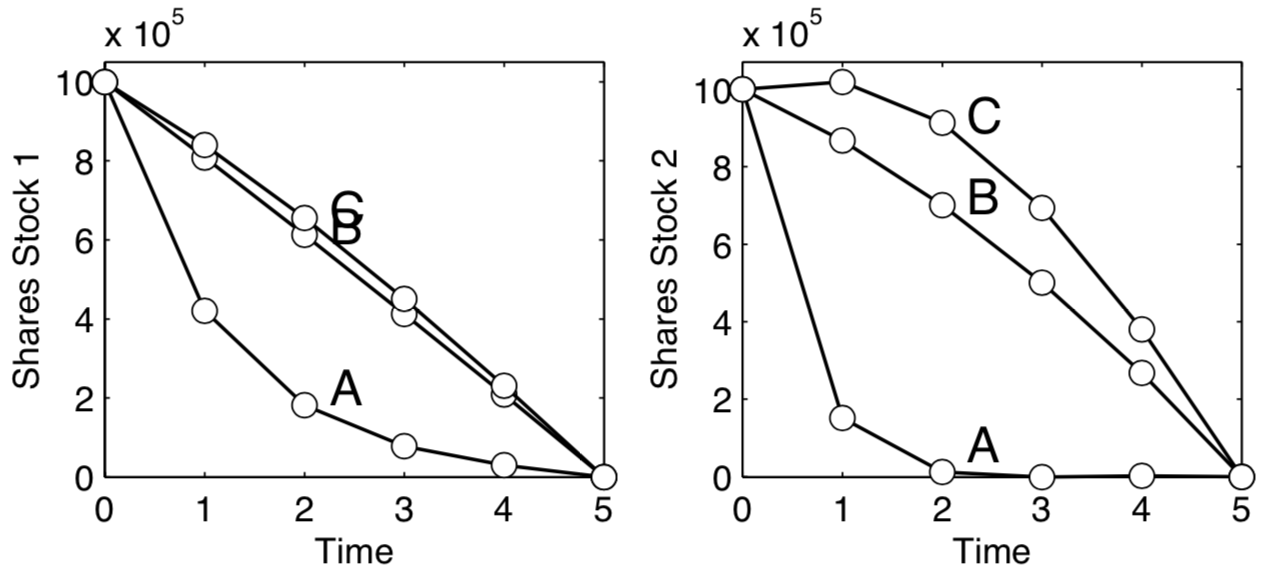
\includegraphics[width=\textwidth]{chapters/chapter_exec_models/figures/opt_traj.png}
	   \caption{Optimal Trajectories for two securities; ($A: \lambda= 2 \times 10^{-6}$; $B: \lambda=0$; $C= -5 \times 10^{-8}$; $B$ is the na\"ive strategy). \label{fig:7first}}
	\end{figure}
	\begin{figure}[!ht] 
	   \centering
	    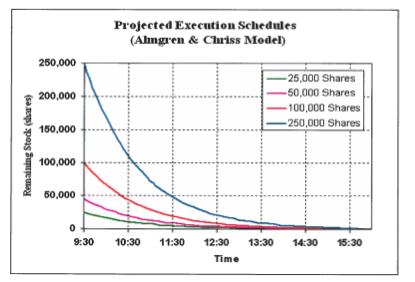
\includegraphics[width=\textwidth]{chapters/chapter_exec_models/figures/temp2.png}
	   \caption{Projected Execution Schedules \label{fig:7second}}
	\end{figure}
Some questions remain: what is the link between market impact and the dynamics of limit order book, is the impact function linear empirically, etc.. The effect of a short term drift in prices and the serial correlation in the errors which is observed in high frequency etc can be incorporated easily in the model (\ref{eqn:morepk}). Lorenz and Almgren (2011) \cite{lovenz2011} provide a Bayesian approach to the optimization problem. While the methodology yields elegant solutions, empirical use of these results require a close monitoring of order book dynamics as the changes in demand and supply sides can be quite rapid. The general behavior of this adaptive strategy is aggressive; it depends on the prediction of short term price change; generally, if price goes up sell faster. 


The above mean-variance formulation of execution cost is combined with the traditional mean-variance portfolio optimization in Engle and Ferstenberg (2007)~\cite{engle2007} and Engle, Ferstenberg and Russell (2012)~\cite{engle2012}. We will discuss this in the context of portfolio rebalancing and the need for minimizing the transaction costs associated with all trades. While the above methods can be taken as first generation methods that are purely based on slippage, more recent work focus on adding other constraints such as incorporating the market VWAP and simultaneously determining the limit and market orders to achieve optimal results. \\


\noindent\textbf{Obizhaeva and Wang Model:} The models discussed in the previous sections assume price impact function that is not sensitive to liquidity dynamics. Obizhaeva and Wang (2013)~\cite{obizhaeva} develop a model that accounts for the dynamic properties of supply and demand as represented in the limit order book. The model captures `resilience'; that is, how the current trade affects the state of the future limit order book. The resulting strategy consists of a large trade initially aimed at moving the order book away from its steady state followed by a number of small trades that will utilize the inflow from new liquidity providers. The speed at which the book replenishes itself is an important part of execution cost. The level of resilience depends on the level of hidden liquidity in the market. The price impact model considered here takes into account the dynamics of the limit order book.


It is assumed that the parent order $X$ will be traded in the interval $(0,T)$, `$n$' times at $t_1,t_2,\ldots,t_n$. To model the execution of a large order in the limit order book, it is assumed that the price of execution ($p_t$) depends on the true value of the equity ($p_t^*$) and the state variables ($z_t$) such as past trades that may affect the book. Let $q(p_t^*,p_t;z_t)$ be the density of the limit orders in the other side of the book. The mid-quote ($\overline{p}_t$) is generally taken to reflect the true price, $p_t^*$. If the trade is on the buy side, the initial large transaction, $x_1$, can push the ask price to a higher level, $p_1^*+(s/2)+(x_1/q)$, where `$s$' is the spread and the average execution price is then equal to $p_1^*+(s/2)+x_1/(2q)$. After the initial execution the price converges to a new steady state, $p_t^*+s/2+\lambda x_1$. Assuming that the limit-order book converges to its steady-state exponentially and at time `$t$', 
	\begin{flalign}\label{eqn:qtdouble}
	&& q_t(p)&= q\cdot I(p>A_t) && \notag \\
	\text{and} && \phantom{x} & \phantom{x} && \\
	&& A_t&= \overline{p}_t + \dfrac{s}{2} + x_1 \cdot \kappa e^{-\rho t}, && \notag
	\end{flalign}
where $A_t$ is the asking price, $\kappa=1/q-\lambda$ and `$\rho$' measures the resilience of the limit order book. If more the current ask price ($A_t$) deviates from steady state level, $\overline{p}_t+s/2$, the new ask limit orders will come into the book as the rate of $\rho \,q (A_t - \overline{p}_t-s/2)$. 


Given the above description of the limit order book dynamics, the optimal execution problem can be restated as follows:
	\begin{equation}\label{eqn:min}
	\min_{x_k} E_1\left(\sum_{k=1}^n [A_k + x_k(2q)]x_k\right),
	\end{equation}
such that $A_k=p_k^*+\lambda(X_1-X_n)+\dfrac{s}{2}+\sum_{i=1}^{k-1} x_i\cdot \kappa e^{- \rho\tau(n-i)}$, where $p_k^*$, the true price is taken to follow a random walk.


The solution to this dynamic programming problem is given in Obizhaeva and Wang (2013, p.14, Proposition 1)~\cite{obizhaeva} and is somewhat involved. Instead we state, the strategy when $n\to\infty$ which is of practical interest as many parent orders are divided into many, many child orders. The empirical market impact study that was presented in the last chapter attests to that. The solution to (\ref{eqn:min}) as $n\to \infty$ are:
	\begin{equation}\label{eqn:orders}
	\begin{split}
	\text{First and final orders}: x_1&= \dfrac{X}{\rho_{T+2}} = x_n  \\
	\text{Spread of in-between trading}: x_t&= \dfrac{\rho x}{\rho_{T+2}}.
	\end{split}
	\end{equation}
The expected cost is determined as
	\begin{equation}\label{eqn:expected}
	\text{Expected cost}=\left(p_0^*+\dfrac{s}{2}\right)X_t+\lambda X_0X_t+\alpha_t X_t^2+\beta_t X_t D_t+\gamma_t D_t^2,
	\end{equation}
where $\alpha_t=\dfrac{\kappa}{\rho(T-t)+2} - \dfrac{\lambda}{2}$, $\beta_t=\dfrac{2}{\rho(T-t)+2}$ and $\gamma_t= - \dfrac{\rho(T-t)}{2\kappa[\rho(T-t)+2]}$. The initial and final orders are discrete in nature and the orders in-between are continuous. They make use of incoming orders with favorable prices. 


Some comments are worth noting. Note the solution given in (\ref{eqn:orders}) does not depend on the market depth, `$q$' and the price impact, `$\lambda$'. It is shown that the price impact is not a factor if the trade times are determined optimally and if they are not set apriori as in the other strategies. The reason for `$q$' not being a factor is due to the fact that the depth is taken to be constant at all times. This implies that there is enough liquidity in the market and the book gets replenished, albeit at a constant rate. The two factors that play important roles are the resiliency factor, `$\rho$' and the trading horizon, `$T$'. When $\rho=0$ the execution costs are strategy dependent and when $\rho\to\infty$, the order book rebuilds itself faster. When `$T$' increases, the size of the first and final order decreases; if there is more time to trade, the trades are spread out to manage the execution cost. The net cost of this strategy is
	\begin{equation}\label{eqn:netcost}
	\text{Net cost}=\dfrac{\lambda}{2} \cdot X^2 + \left(\dfrac{\kappa}{\rho_{T+2}}\right)^2 X^2
	\end{equation}
and it is shown to be smaller than the cost incurred if the strategy of constant rate trading is followed. 


Obizhaeva and Wang (2013)~\cite{obizhaeva} consider the extension of the optimization criterion in (\ref{eqn:min}) to include the risk aversion as well, as in Almgren and Chriss (2000)~\cite{alm2000}. Interested readers should refer to Section~8 their paper. For a practical implementation of these methods, it is necessary to consider the trading that happens in multiple exchanges and how the replenishment patterns can differ over different exchanges where `liquidity' and the fee structure have become major considerations for the order flow. 


\noindent\textbf{Easley, De Prado and O'Hara Model:} In the models described so far in this section, it is assumed that the number of child orders `$n$' and the execution horizon, `$T$', are decided exogenously. Also the impact of a trade is modeled through the modified random walk model for the price with additional terms reflecting the permanent or temporary impact (Equation (\ref{eqn:pk7}), (\ref{eqn:bigpk}) and (\ref{eqn:pdouble})). The process of how price impact arises due to friction in the liquidity access is an important part of market microstructure theory and this needs to be taken into account in determining the optimal execution. For example, a buyer in a seller's market can incur a lower cost of trading than a seller in a similar market. Obizhaeva and Wang model is based on the arrival dynamics to the order book. 


The approach taken by Easley, De Prado and O'Hara (2015)~\cite{prado2} is based on an asymmetric information model of the market maker's behavior. The key measure is the probability of information-based (PIN) trading that is estimated by the order book imbalance (see Easley, De Prado and O'Hara (2012)~\cite{prado3}). Selling a large order in a market already imbalanced toward sell, will reinforce adverse selection from the other side and thus widen the bid-ask spread resulting in higher market impact. The optimal execution horizon (OEH) model in Easley et al (2015) provide a framework for determining the trading horizon, `$T$', and does complement other earlier studies on execution strategies that minimize the price impact. 


The PIN that was developed in a series of papers (see Easley, Kiefer, O'Hara and Paperman (1996)~\cite{paper} and the references therein) views trading as a sequential game between liquidity providers and liquidity takers, repeated over the trading duration. If the information about the asset occurs with probability $\alpha$ and the chance that the information is good, is denoted by, $(1-\delta)$ and further assume that the informed traders, who knew the terminal value of the asset under good news ($\overline{S}$) and under bad news ($\underline{S}$) arrive at the rate, $\mu$, and the noise traders arrive at the rate of `$\epsilon$'. The PIN is approximated as (assuming $\delta=1/2$)
	\begin{equation}\label{eqn:pin}
	\text{PIN}=\dfrac{\alpha\mu}{\alpha\mu+2\epsilon} \sim E[\text{OI}]
	\end{equation}
where order imbalance (OI), ($\text{OI}=\frac{V^B-V^S}{V}$), with $V$ denoting the volume. An aggressive buy order of size `$m$' can affect the order imbalance as
	\begin{equation}\label{eqn:oi}
	\text{OI}=\left(2 \cdot \dfrac{V^B}{V}-1\right)\left(1-\dfrac{m}{V}\right) + \dfrac{m}{V},
	\end{equation}
and note that $\left(2\cdot \frac{V^B}{V}-1\right)$ is the order imbalance, when $m=0$, that is without the large trade. When `$m$' is small, the OI is likely to be perturbed too much and $m \to V$, that is the buy order will take all the available liquidity, then OI$\to1$. This also indirectly quantifies the amount of leakage or signaling that occurs with each trade.


An important factor that is associated with PIN is the range of liquidity that may exist in the market in the presence of both informed and noise traders:
	\begin{equation}\label{eqn:newsigma}
	\Sigma = \text{PIN} \cdot [\overline{S} - \underline{S}]
	\end{equation}
slicing a large order into small orders as suggested by earlier execution strategies does have timing risk and the asset price is assumed to follow a random-walk resulting in:
	\begin{equation}\label{eqn:randomwalk}
	\Delta S=\sigma \sqrt{\dfrac{V}{V_\sigma}} \, \xi,
	\end{equation}
where $\xi \sim N(0,1)$, $V_\sigma$ is the volume in the mid-price range. With `$\lambda$' as the probability of accepting a loss greater than $z_\lambda \cdot \sigma \cdot \sqrt{V/V_\sigma}$, the loss from trade size, `$m$', can be shown to be bounded by,
	\begin{equation}\label{eqn:bigbracp}
	P \left[ \dfrac{m \cdot \Delta s}{\hat{\sigma} \sqrt{\dfrac{V}{V_\sigma}}} > z_\lambda \right] = 1-\lambda
	\end{equation}
and thus `$\lambda$' can be interpreted as a `risk aversion' parameter. The OEH's goal is to determine the optimal trading volume, $V$, that can hide the purported trade, $m$, with minimum timing risk. The probabilistic loss function $\Pi$ that incorporates both liquidity and timing risk component is defined as:
	\begin{equation}\label{eqn:pi}
	\Pi = \left| \varphi(m) \cdot \text{OI} + (1-\varphi(m)) (2V^B-1)(\overline{S}-\underline{S})\right| - z_\lambda \sqrt{\dfrac{V}{V_\sigma}} \, \sigma.
	\end{equation}
Here $\varphi(m)$ is a monotonic function that maps into the range $(0,1)$. If `$V$' is greater, its impact is smaller in OI and larger in the trading range. The optimization results are given in Easley et al (2015)~\cite{prado2}.


The key quantities in determining the OEH are the order imbalance and the trade size/side. Figure~\ref{fig:3temp}, reproduced from Easley at al demonstrates how selling in a buyer's market allows for shorter horizons and in seller's market leads to longer horizons.  


\begin{figure}[!ht] 
   \centering
    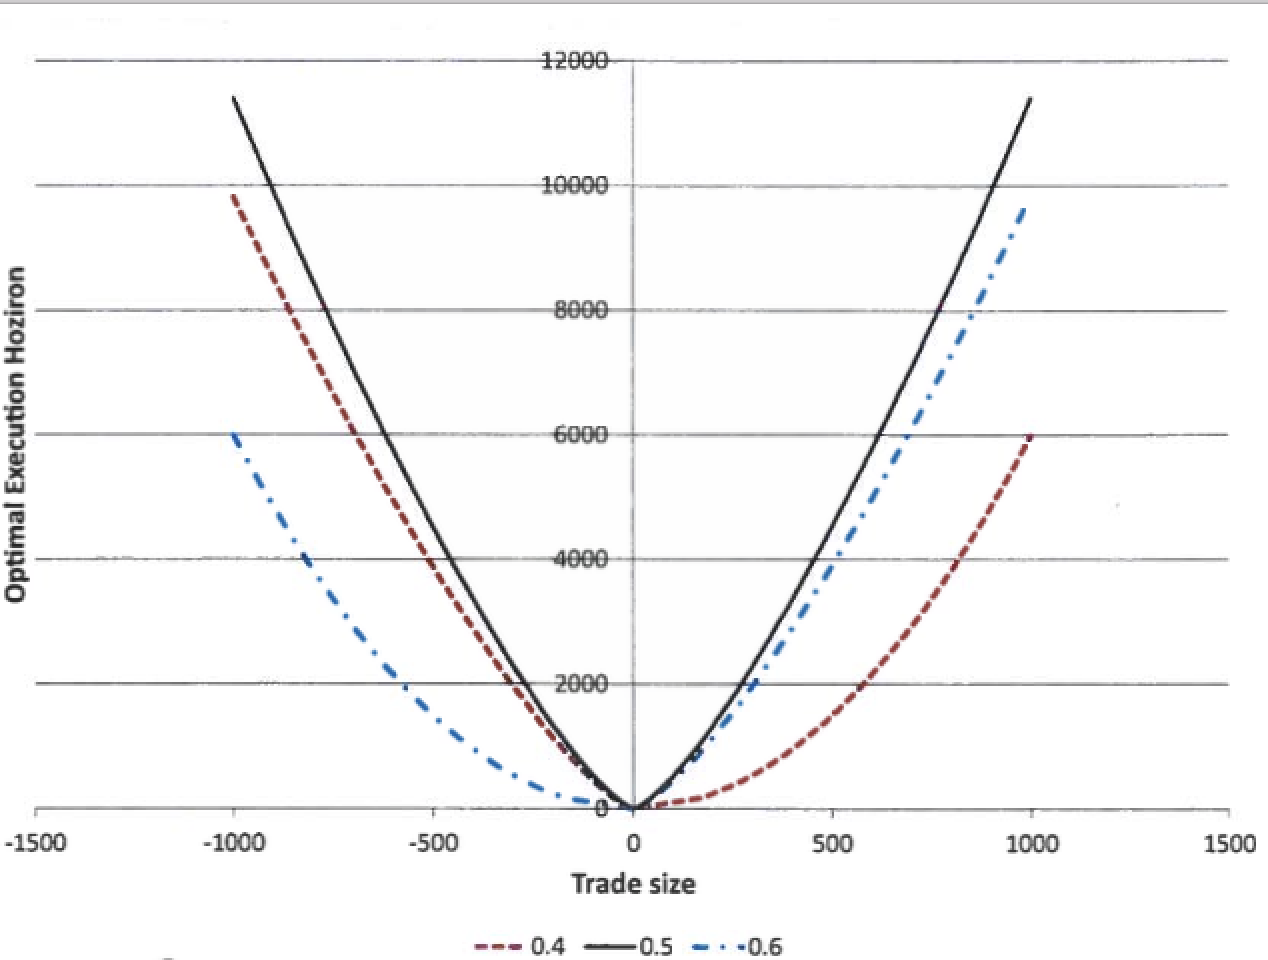
\includegraphics[width=\textwidth]{chapters/chapter_exec_models/figures/fig3temp.png}
     \caption{Optimal execution horizons for various order imbalances and trade sizes/sides. Combining alternative trade sizes and sides with our three scenarios ($v^B=0.4$, $v^B=\frac{1}{2}$, $v^B=0.6$) results in the optimal execution horizons displayed in the figure above, $\hat{\sigma}=1,000$, $V_\sigma=10,000$, $m=1,000$, $[\overline{S}-\underline{S}]=10,000$, $\lambda=0.05$ and $\varphi[|m|]$ linear. \label{fig:3temp}}
\end{figure}



\section{Multiple Exchanges:  Smart Order Routing}

In the USA there are over ten lit venues and close to forty dark venues and thus equity markets are highly fragmented. Each venue functions as an electronic limit order book of its own, where orders are prioritized first based on their prices and then at a given price level, according to their time of arrival. Exchanges publish information for each security in real-time and the information can change rapidly due to cancellations. The exchanges may differ with respect to best bid and offer price levels, the market depth at various prices etc. The exchanges also differ in their fee structures. Under the maker-taker pricing, exchanges offer rebates to liquidity providers and charge fees to takers of liquidity. These fees can range from $-\$0.001$ to \$0.0030. Because the typical bid-ask spread is \$0.01, the fees and rebates are a fairly significant fraction of the trading costs. Thus market participants must decide where child orders should be sent. It may be expensive to route to all the exchanges and by not routing to the right venue, it is possible to miss liquidity and hence incur greater market impact. At any point in time, the highest bid and the lowest offer among all exchanges comprise the National Best Bid and Offer (NBBO). Most traders use the smart order routing algorithms with goal to buy or sell the maximum number of shares in the shortest possible time with the least market impact possible. But a key issue is that many of the lit venues have hidden orders (12--45\%). How to estimate the size of the hidden orders and how to make routing decisions in the presence of hidden orders has been a focus of some recent research studies.


While exchanges compete along many fronts, for example, payment for order flow, transparency and execution speed, the key variables driving the efficiency are liquidity and price improvement. Thus the design of market structure is considered by market participants and regulators as the key determinant of flow of liquidity. The coexistence of multiple exchanges as mentioned in Parlour and Seppi (2003)~\cite{parlour2003} raises specific questions that are stated below:
\begin{enumerate}[a)]
\item Do liquidity and trading concentrate in a few exchanges?
\item Do some market designs provide greater liquidity than others?
\item Is the fragmentation of order flow desirable from a policy point of view?
\item What is the constructive role for regulators to enhance liquidity?
\end{enumerate}


Because exchanges operate under rules governing certain market designs, the performance and efficiency issues are related to the types of markets, such as pure limit order and a hybrid market (limit order book plus a specialist). In the hybrid market a specialist can provide supplementary liquidity after a market order has arrived. Parlour and Seppi (2003)~\cite{parlour2003} conclude only under some conditions such as enforcement of time priority, the efficiency is possible. Merely increasing the number of trading venues may result in degradation of market quality, if the enforcement of time priority is not followed, as it might discourage traders from posting the limit orders.


Foucault and Menkveld (2008)~\cite{foumen}consider the effect of fragmentation on two limit order markets. They examine the competition between Euronext and London Stock Exchange (LSE) in the Dutch market. The consolidated limit order book is found to be deeper after entry of the LSE. General conclusions from the above study and others such as Hendershott, Jones and Menkveld (2011)~\cite{hjm} and O'Hara and Ye (2011)~\cite{oye} are that fragmentation of order flows improves the liquidity supply and protecting orders against trade-throughs is important. Thus multiple exchanges are here to stay and smart order routing algorithms that can work well with the increased number of exchanges would be favorably sought by the market participants.


The smart order router (SOR), generally works as follows. A user can customize the use of the strategy by establishing a set of rules in splitting the parent order into child orders and the smart order routers are designed to ensure that the orders are routed to the venue with the best price and the orders are filled according to the trading strategies that may be pre-determined or may be adaptive. To be successful, SORs must be able to handle a variety of trading strategies and multiple venues. In addition they must deal with vast amount of incoming and historical market data. The publicly available information on the SORs used by major traders indicate that the order placement objective in general is to minimize client all-in shortfall with or without venue fees. The all-in shortfall consists of the shortfall on the filled shares and the cost of the clean-up trade for the unfilled shares. The latter is taken to be an important component of order placement optimization as it enables to quantify the effect of venue differences in fill rates, (see Street Smart, Issue 42, Jan 14, 2011). Other programs used in industry chose to optimize the expected time to execute the client's overall order. Expected queue speeds at various venues are predicted from recent trading data. Small orders tend to be placed in a single venue to minimize the queueing time whereas large orders will be placed in multiple venues to access maximum liquidity. In this model forecasting trading rates at different venues is crucial for successful implementation of the program. The rates are modeled as a function of lagged rates, thus capturing the momentum, and imbalances between supply and demand sides of the order book. Thus order placement in a fragmented market is not a trivial task.


A recent empirical study by Battalio, Corwin and Jennings (2016)~\cite{battcorjen} confirms that brokers use both limit and marketable orders to execute trades. Past studies provide evidence that market orders are sent to venues with lower trading costs and the trading fees and rebates generally affect consolidated market depth. Maglaras, Moallemi and Zheng (2012)~\cite{magmoazhe} show that limit orders are submitted to exchanges with high rebates and lower waiting time for execution while market orders are sent to venues that have lower fees and larger posted quote sizes. Cont and Kukanov (2017)~\cite{contk} develop a model that is somewhat more realistic to the current practice by decoupling the `order placement' decision from the scheduling decision and more importantly consider the option of placing limit orders on several exchanges, simultaneously. The model also accounts for the execution risk, the risk of not filling an order. Filling the unfilled portion may be costly and the allocation may shift toward market orders or toward overbooking, that is placing more orders than needed to refill.


To formalize the order placement problem, we assume a size of order $X$ is to be filled in the duration $(0,T)$. The decision is to split this order into a market order $M$ and `$K$' limit orders $L_1,\ldots,L_K$ with the same size to be placed in `$K$' exchanges with queue sizes $Q_1,\ldots,Q_K$ ; thus the order allocation is summarized by the elements of the vector $X=(M,L_1,\ldots,L_K)$ that need to be optimally determined. If order cancellations in the duration $(0,T)$ in exchange `$K$' is represented by $\xi_K$, then the number of shares transacted can be written as 
	\begin{equation}\label{eqn:axe}
	A(X,\xi)= M + \sum_{k=1}^K \left[ (\xi_k - Q_k)_+ - (\xi_k - Q_k - L_k)_+ \right],
	\end{equation}
where the terms in the parenthesis refers to the initial position and the final position of the queue outflows. The execution cost must account for fee ($f$) and rebate structures (discussed in Chapter~\ref{chap:ch_mi_models}) in each exchange and the cost of adverse selection ($r_k$) and can be stated as follows:
	\begin{equation}\label{eqn:cxe}
	C(X,\xi)= (h+f)M - \sum_{k=1}^K (h+r_k) \left[ (\xi_k - Q_k)_+ - (\xi_k - Q_k - L_k)_+ \right].
	\end{equation}
Here $h$ is one-half of bid-ask spread. 


The cost function in (\ref{eqn:cxe}) can be modified to account for the cost of unfilled limit orders which may be filled through market orders at higher cost or it is possible that the prices have decreased resulting in additional adverse selection cost with penalty ($\lambda_u$) for falling behind and penalty ($\lambda_0$) for exceeding the target; Thus, the execution risk can be written as,
	\begin{equation}\label{eqn:er}
	\text{ER}= \lambda_u (S-A(X,\xi))_+ + \lambda_0 (A(X,\xi)-S).
	\end{equation}
To be more realistic, the market impact function can be considered as follows:
	\begin{equation}\label{eqn:mi}
	\text{MI}= \theta \left[ M + \sum_{k=1}^K L_k + (S-A(X,\xi))_+ \right].
	\end{equation}
The total cost function that includes both implicit and explicit costs can be states as:
	\begin{equation}\label{eqn:vxe}
	V(X,\xi)= C(X,\xi) + \text{ER} + \text{MI}.
	\end{equation}
The random variable in (\ref{eqn:vxe}) is $\xi$, the cancellations that occur in various exchanges and the minimization function is $E[V(X,\xi)]$ with some assumed distribution for $F$ of $\xi$. Under some reasonable assumptions such as that the trader will not execute more than the target $X$ and market orders in the beginning of the duration $(0,T)$ are less expensive than at the end when unfilled orders are converted to market orders, an optimal solution is shown to exist (see Cont and Kukanov (2017)~\cite{contk} for details).


The analytical solution minimizing $V(X,\xi)$ is not easily tractable due to dimensionality issues. A numerical solution via gradient method is proposed. Random samples of $\xi$ are obtained and averaged to approximate $E(\xi)$. Let $q(X,\xi)= \Delta V(X,\xi)$ be the gradient of $V$. The following iterative algorithm is shown and converges:
	\begin{enumerate}[--]
	\item \textbf{Start with }$\mathbf{X_0}$\textbf{ and for }$\mathbf{n=1,2,\ldots,N}$\textbf{ do}
	\item $\mathbf{X_n=X_{n-1} - \gamma_N g(x_{n-1}, \xi^n)}$
	\item \textbf{End; }$\mathbf{X_N^* = \frac{1}{N} \sum_{n=1}^N X_n}$
	\end{enumerate}
The step size, \small
	\begin{equation}\label{eqn:7gammaN}
	 \gamma_N = \sqrt{k} S \left( N(h+f+\theta+\lambda_u +\lambda_0)^2 _ t + N \sum_{k=1}^K (h+r_k+\theta+\lambda_u+\lambda_0)^2 \right)^{-1/2} 
	\end{equation}
\normalsize can be seen as a function of all the costs associated with the execution of the order.

To summarize, recall that the algorithm needs the following input:
	\begin{enumerate}[--]
	\item Trading Costs: 
		\begin{itemize}
		\item One half of bid-ask spread ($h$)
		\item Market order fee ($f$)
		\item Effective limit order risks ($r_k$)
		\item Market impact coefficient ($\theta$)
		\item Penalties for overfilling or underfilling ($\lambda_0,\lambda_u$)
		\end{itemize}
	\item Market Variables: Number of exchanges ($K$) and limit order queues ($Q_k$).
	\item Execution Variables: Time horizon ($T$) and target quantity ($S$).
	\end{enumerate}
While many of these quantities can be estimated using past transactions, the limit order queues ($Q_k$) and the cancellations ($\xi_k$) are to be obtained at the time of execution.



\section{Execution Algorithms for Multiple Assets}

The execution of trading entry-exit decisions can be made using the methods described in the earlier section for individual assets. Most investors hold multiple assets in their portfolios and evaluate their investments as a whole rather than in parts. In Section~\ref{sec:port_trad_strat}, we discussed the trading strategies with the focus on rebalancing the portfolios. The criteria used were in the traditional framework of mean-variance efficiency with some constraints on the transaction costs. When it comes to execution, the criteria as noticed from earlier sections is on execution costs and the market impact. We will briefly outline some models presented in the literature for multiple-security portfolios.


Only recently there are efforts made to better understand and model cross-impact of trading an asset on trading of related assets. If a trader is liquidating simultaneously multiple assets as part of the rebalancing effort, we should expect some cross-impact. In the low frequency setting this is studied under `commonality' or `co-movement' as discussion in Chapter~\ref{ch:ch_mvts}. In the high-frequency setting, the problem is harder to study due to short-term market frictions. 

























\section{Multiple Stocks: Microstructure Issues}
\section{A Stochastic Adaptive Control Approach to Optimal Execution}
\section{Algorithmic Trading Next Frontiers}
\subsection{Extending the Algorithms to Derivative markets}
\subsection{Developing a Trading Platforms for Simultaneous Execution of Assets}
\subsection{Future of Algorithmic Trading}